%% %%%%%%%%%%%%%%%%%%%%%%%%%%%%%%%%%%%%%%%%
%% main.tex
%% Hauptdatei für content
%% %%%%%%%%%%%%%%%%%%%%%%%%%%%%%%%%%%%%%%%%
%\begin{abstract}
%\noindent
%\end{abstract}


%--------
% Wer macht was?
% V: Anfang & "Where are we?" & Table of Contents
% T: Quick Reminder
% V: Kernel estimate
% T: kNN
% V: Comparison
% T: Programmierteil
%--------

\begin{frame}
\frametitle{Where are we?}
\begin{tabularx}{0.98\textwidth} {
  | >{\centering\arraybackslash}X 
  || >{\centering\arraybackslash}X
  | >{\centering\arraybackslash}X 
  | >{\centering\arraybackslash}X | }
 \hline
   & \textbf{Partitioning} & \textbf{Kernel} & \textbf{k-NN} \\ 
 \hline
 \hline
    \textbf{weak} & & & \\
    universal consistency & \checkmark & \checkmark & \checkmark \\
 \hline
    \textbf{strong} & & & \\
    (universal) consistency & \checkmark & \textbf{?} & \textbf{?} \\ 
 \hline
\end{tabularx}

\end{frame}

\begin{frame}
\frametitle{Table of Contents}
\tableofcontents
\end{frame}

\section{Quick reminder}

\begin{frame}
\frametitle{Kernel \& k-NN estimate}
\begin{block}{Definition (kernel estimate)}
    \[m_n(x) = \frac{\sum_{i=1}^nK(\frac{x-X_i}{h})Y_i}{\sum_{i=1}^nK(\frac{x-X_i}{h})}\]
\end{block}
\begin{block}{Definition (k-NN estimate)}
    \[m_n(x) = \frac{1}{k} \sum_{i=1}^kY_{(i)}(x)\]
\end{block}    
\end{frame}

\begin{frame}
\frametitle{Strong (universal) consistency}
\begin{block}{Definition (Strong (universal) consistency)}
    \underline{Strong consistency}
    \[\limn \int \abs{m_n(x) - m(x)}^2 \mu(\diff{x}) = 0 \quad\text{with probability one.}\]
    
    \underline{Strong universal consistency}
    \[\limn \int \abs{m_n(x) - m(x)}^2 \mu(\diff{x}) = 0\]
     for all distributions of $(X,Y)$ with $\ev{Y^2}<\infty$.
\end{block}
\end{frame}

%---------------

\section{Kernel Estimates}

\begin{frame}
\frametitle{Regular kernels}

\begin{block}{Definition (regular kernels)}
Kernel $K$ \textbf{regular}: $\Longleftrightarrow$ \\
$K$ is non-negative and $\exists$ $B_r(0)$ with $r>0$ and $b>0$, such that \[ 1 \geq K(x) \geq b \ind{\{x \in B_r(0)\}} \] and \[\int \sup\limits_{u \in x+B_r(0)} K(u) \dx < \infty. \]
\end{block}
\begin{figure}
    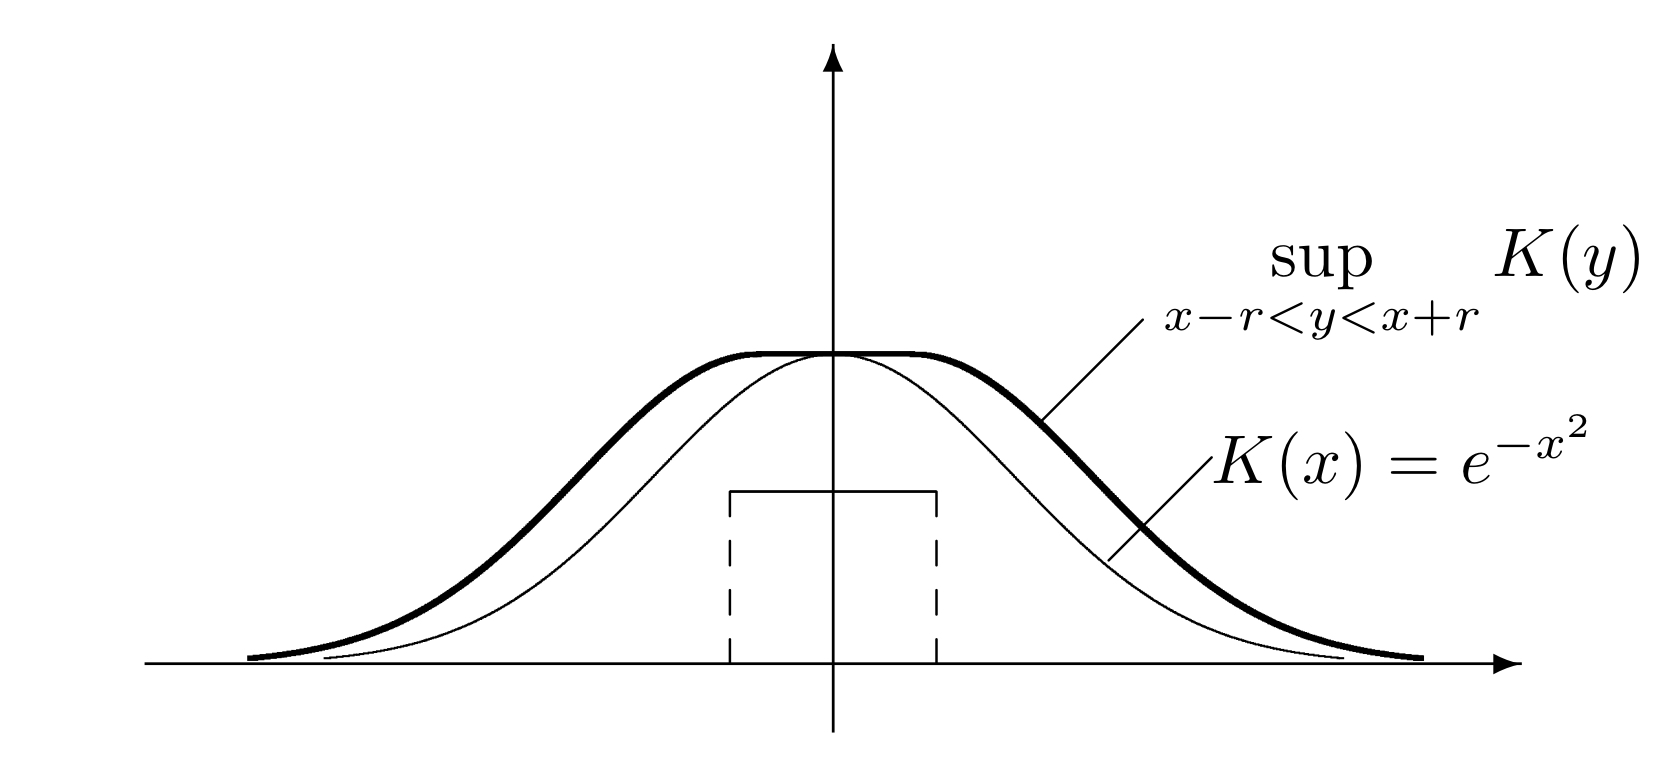
\includegraphics[scale=0.085]{regularKernelFigure.jpeg}
    \centering
\end{figure}
\end{frame}

\begin{frame}
\frametitle{Strong consistency of the kernel estimate}
\begin{alertblock}{Theorem 2.1 (strong consistency)}
Let $m_n$ be the kernel estimator of the regression function $m$ with a regular kernel K. Assume $\exists L<\infty$: $P(|Y| \leq L) = 1.$ \\ If \[h_n \to 0 \quad and \quad nh_n^d \to \infty,\] then the kernel estimate is \textbf{strongly consistent}.
\end{alertblock}
\end{frame}

\begin{frame}{Proof components (overview)}
\begin{figure}
    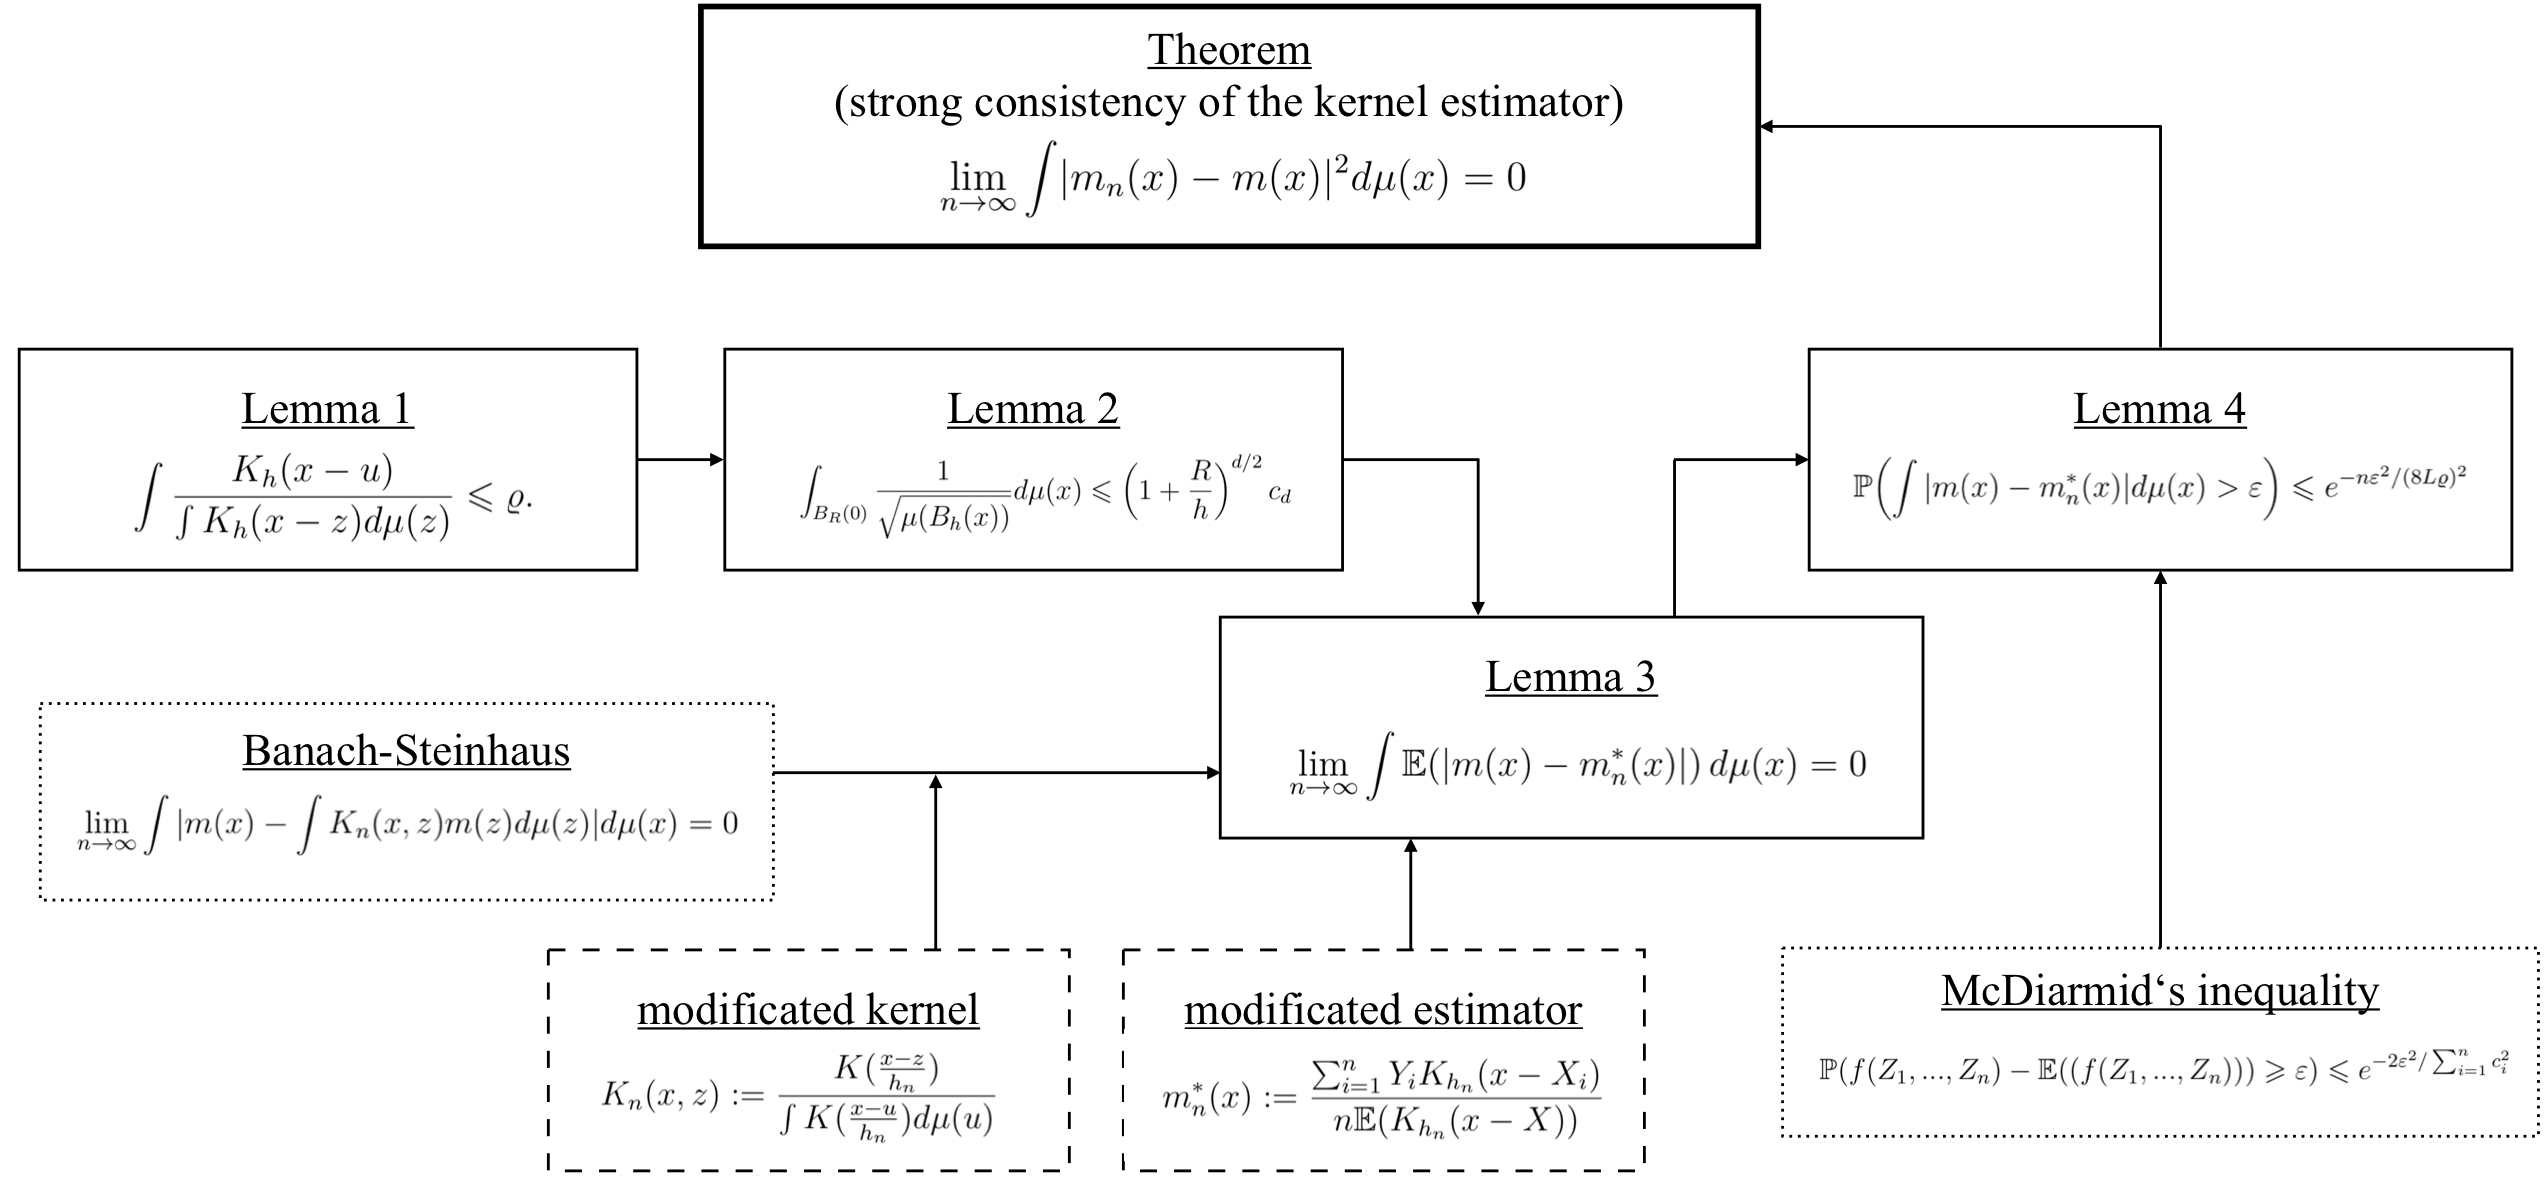
\includegraphics[scale=0.11]{organigramkernel.jpeg}
    \centering
\end{figure}
\end{frame}

\begin{frame}
\frametitle{Proof Components 1}
\begin{block}{Lemma 2.1 (Covering Lemma)}
Kernel $K$ is regular. $\Longrightarrow$ \\
$\exists \rho \equiv \rho(K)<\infty$, such that $\forall u \in \mathbb{R}^d$, $h>0$ and probability measure $\mu$ \[\int \frac{K_h(x-u)}{\int K_h(x-z) \mu(dz)} \mu(\dx) \leq \rho.\]
Moreover, $\forall \delta > 0$ \[\lim_{n\to\infty} \sup\limits_{u \in \mathbb{R}^d} \int \frac{K_h(x-u) \ind{\{ \| x-u \| > \delta \} }}{\int K_h(x-z) \mu(dz)} \mu(\dx) = 0.\]
\end{block}
\end{frame}

\begin{frame}
\frametitle{Proof Components 1}
\begin{figure}
    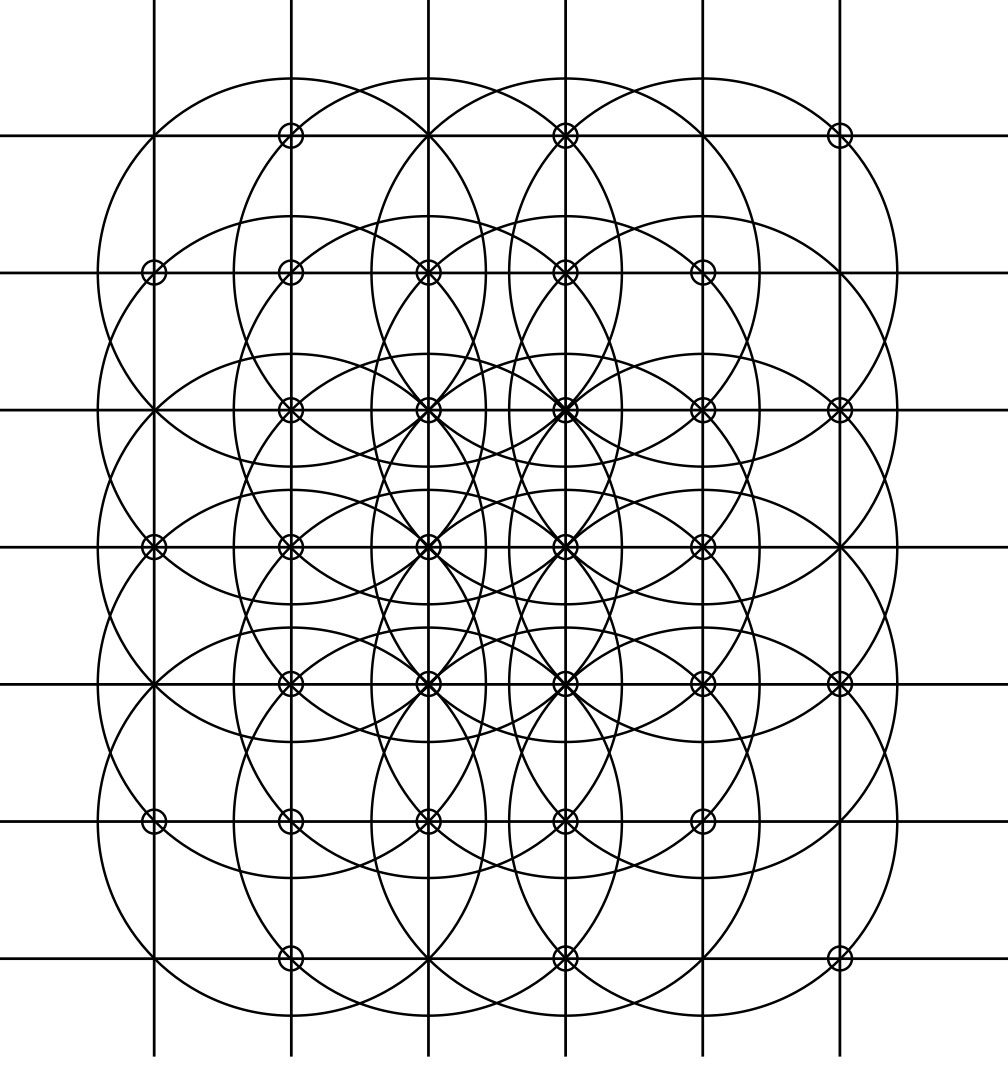
\includegraphics[scale=0.11]{coverofR2.jpeg}
    \caption{An example of a bounded overlap of $\R^2$.}
    \centering
\end{figure}    
\end{frame}

\begin{frame}
\frametitle{Proof Components 2}
\begin{block}{Lemma 2.2}
Let $1 \leq R<\infty$, $0 < h \leq R$, $B_R(0) \subseteq \mathbb{R}^d$ ball of Radius $R$. $\Longrightarrow$ \\
For every probability measure $\mu$, \[\int_{B_R(0)} \frac{1}{\sqrt{\mu(B_h(x))}} \mu(\dx) \leq \left(1+\frac{R}{h}\right)^{d/2} c_d,\] where $c_d$ depends upon the dimension d only.
\end{block}
\end{frame}

\begin{frame}{Proof components 3}

    \begin{center}
        \begin{tikzpicture}
            \node[anchor=south west,inner sep=0] at (0,0) {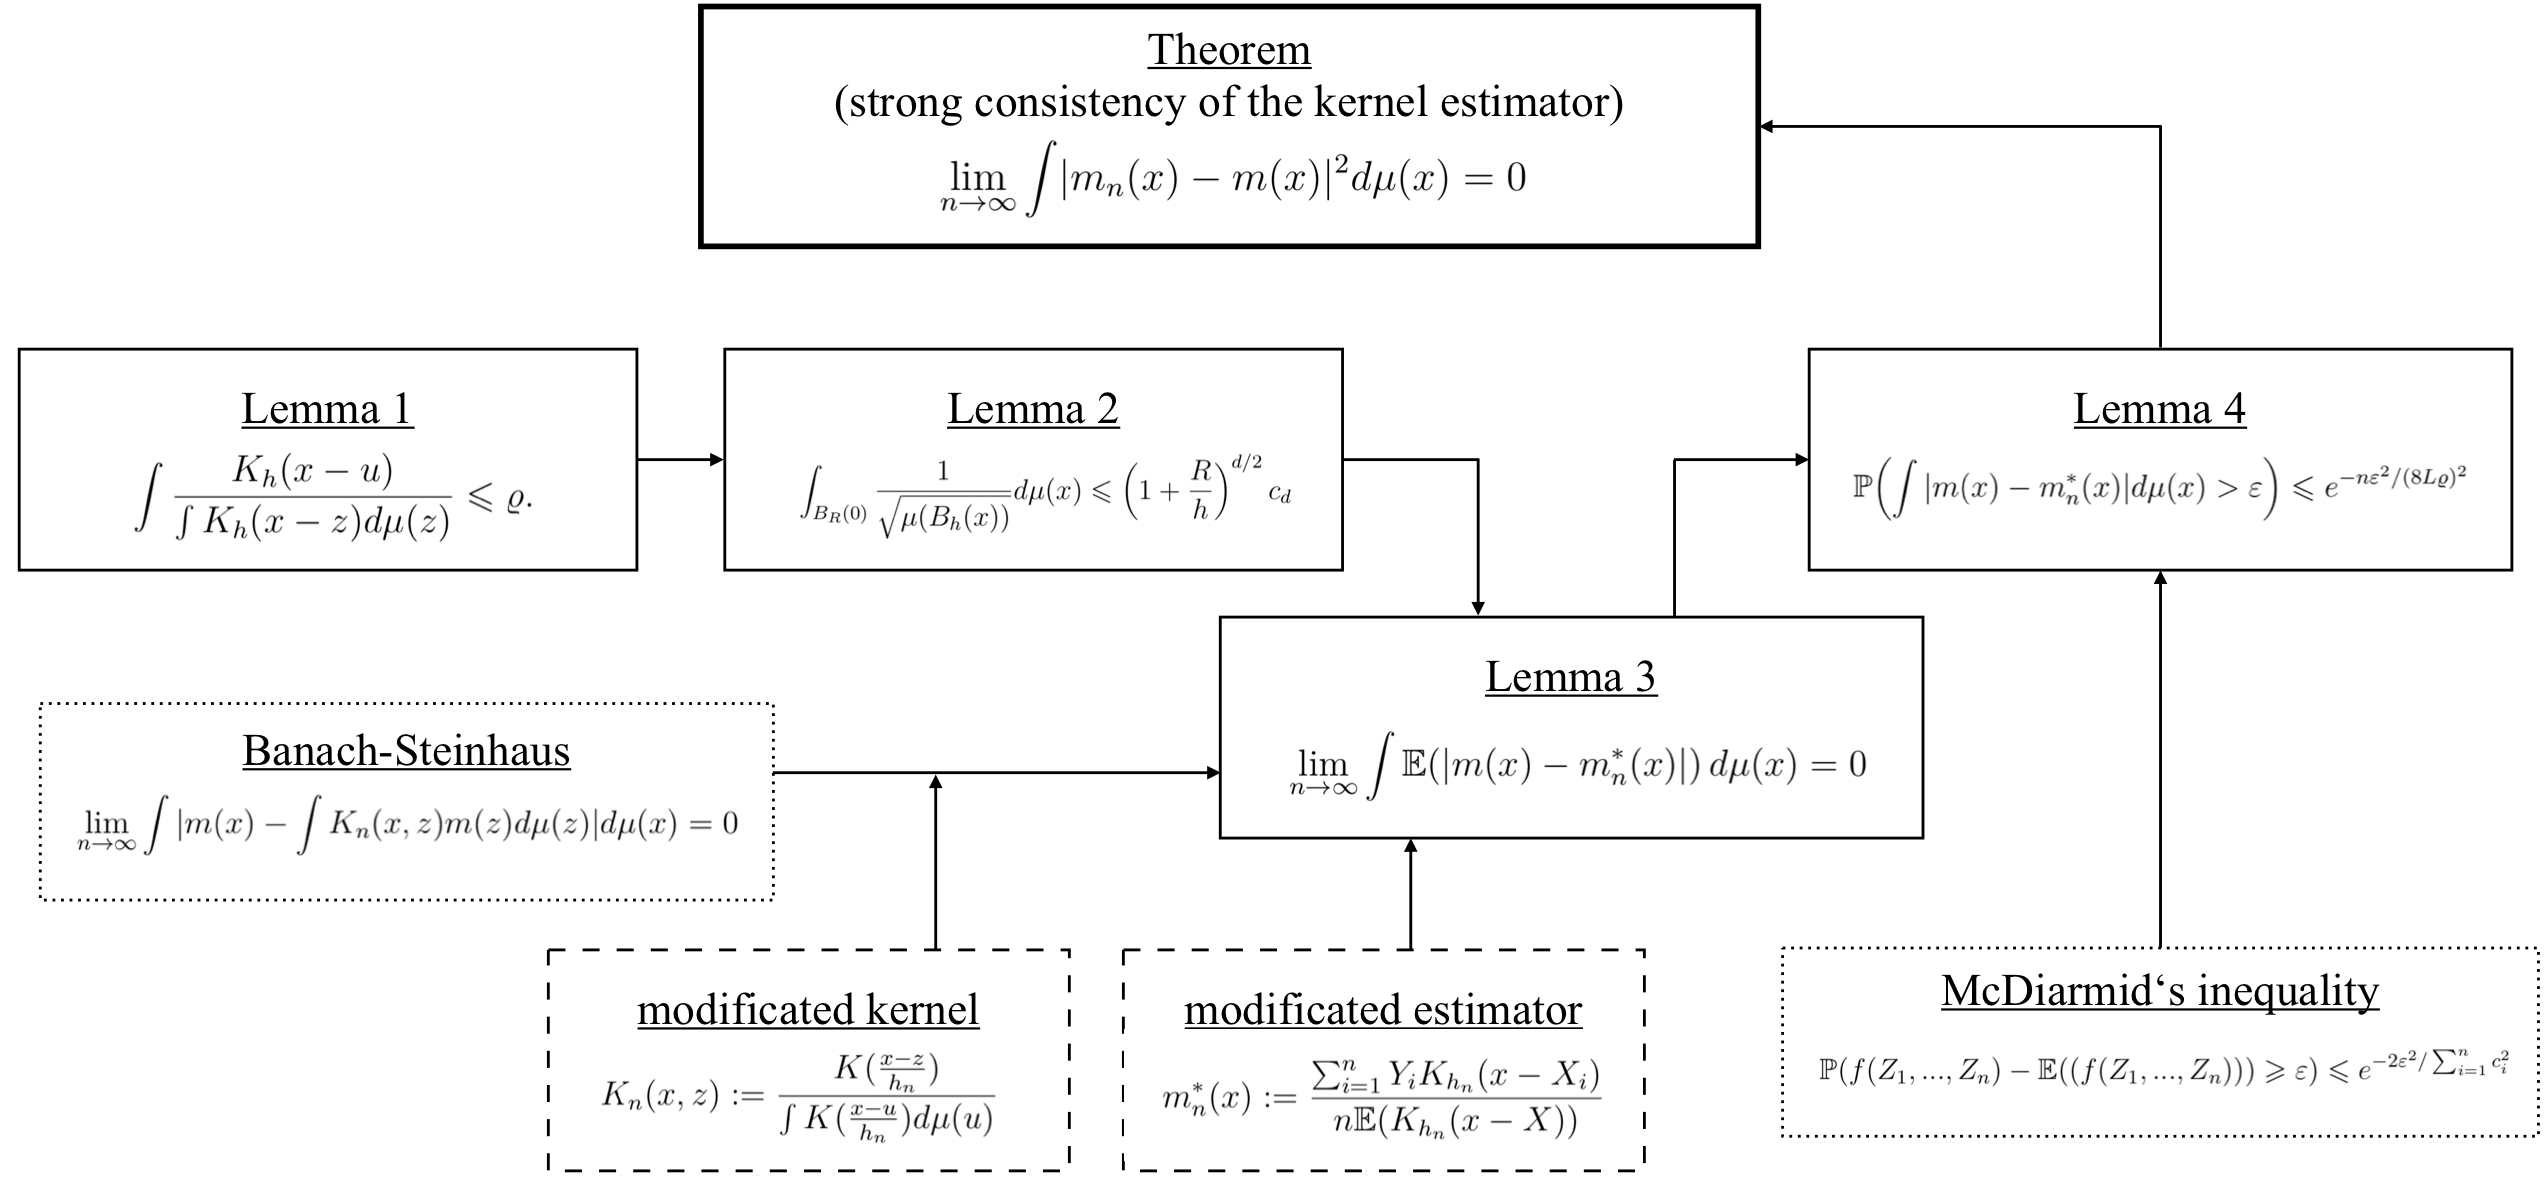
\includegraphics[width=1.3\textheight]{organigramkernel.jpeg}};
            \draw<1>[red,ultra thick,rounded corners] (0,-0.1) rectangle (7.85,2.4);
        \end{tikzpicture}
    \end{center}

\end{frame}

\begin{frame}
\frametitle{Proof Components 3}

\begin{block}{Definition (modificated estimate)}
Define \[m_n^*(x) := \frac{\sum_{i=1}^{n} Y_i K_{h_n}(x-X_i)}{n \ev{K_{h_n}(x-X)}}. \]  
\end{block}
\begin{block}{Lemma 2.3}
Under the conditions of Theorem 1,
\[\lim_{n\to\infty} \int \ev{|m(x) - m_n^*(x)|} \mu(\dx) = 0.\]
\end{block}
\end{frame}

\begin{frame}
\frametitle{Proof Components 3}

\begin{block}{Definition (modificated kernel-function)}
Define \[K_n(x,z) := \frac{K(\frac{x-z}{h_n})}{\int K(\frac{x-u}{h_n}) \mu(\diff{u})}.\]  
\end{block}
\begin{block}{Theorem of Banach-Steinhaus}
\begin{enumerate} [label=(\roman*)]
    \item $\exists c>0$ $\forall n$: $\int |K_n(x,z)| \mu(\diff{x}) \leq c
        \text{   for $\mu$-almost all $z$}$
    \item $\exists D \geq 1$ $\forall n,x$: 
        $\int |K_n(x,z)| \mu(\diff{z}) \leq D.$
    \item $\forall a>0$,
        $ \lim\limits_{n \rightarrow \infty} \int \int |K_n(x,z)| \ind{\{ \norm{x-z} > a\}} \mu(\diff{z}) \mu(\diff{x}) = 0. $
    \item $\lim\limits_{n \rightarrow \infty} \text{ess}\sup\limits_{x} | \int K_n(x,z) \mu(\diff{z})     -1 | = 0.$
\end{enumerate}
$\Longrightarrow$ $ \forall m \in L_1(\mu)$: \\
$\quad \quad \quad \lim\limits_{n \rightarrow \infty} \int | m(x) - \int K_n(x,z)m(z) \mu(\diff{z}) | \mu(\diff{x}) = 0.$
\end{block}

\end{frame}

\begin{frame}
\frametitle{Proof Components 4}
\begin{block}{Lemma 2.4}
For n large enough: \[\pro{\int |m(x) - m_n^*(x)| \mu(\dx) > \epsilon} \leq e^{-n\epsilon^2/(8L\rho)^2}. \]
\end{block}
\begin{block} {Theorem (McDiarmid's Inequality)}
    Let $Z_1,...,Z_n \in A$ be indep. RV and assume for $f:\: A^n \rightarrow \R$:
    \[
        \sup\limits_{z_1,...,z_n,\hat{z_i} \in A} |f(z_1,...,z_n) - f(z_1,...,z_{i-1},\hat{z_i}, z_{i-1},...,z_n)| \leq c_i.
    \]
    Then, $\forall \epsilon > 0$,
    \[
        \pro{f(Z_1,...,Z_n) - \ev{f(Z_1,...,Z_n)} \geq \epsilon} \leq e^{-2\epsilon^2/\sum_{i=1}^n c_i^2}.
    \]
\end{block}
\end{frame}

\begin{frame}{Proof components 5 \checkmark}
$\int |m_n(x)-m(x)| \mu(\diff{x})$ \\
$\quad\quad\quad \leq \underset{\Downarrow}{\underbrace{\int |m_n(x)- \mathbf{m_n^*(x)} | \mu(\diff{x})}} + \underset{Lemma \: 4 \: \: \checkmark}{\underbrace{\int | \mathbf{m_n^*(x)} -m(x)| \mu(\diff{x})}}$
\fbox{\begin{minipage}{27em}
$\quad |m_n^*(x)-m_n(x)| \\
&= \abs[\bigg]{\frac{\sum Y_i K_{h_n}(x-X_i)}{n\ev{K_{h_n}(x-X)}} - \frac{\sum Y_i K_{h_n}(x-X_i)}{\sum K_{h_n}(x-X_i)}} \quad\text{(by definition)}\\
&= \abs[\Big]{\sum Y_i K_{h_n}(x-X_i)}
\abs[\bigg]{\frac{1}{n\ev{K_{h_n}(x-X)}} - \frac{1}{\sum K_{h_n}(x-X_i)}} \\
&\leq L \abs[\Big]{\sum K_{h_n}(x-X_i)}
\abs[\bigg]{\frac{1}{n\ev{K_{h_n}(x-X)}} - \frac{1}{\sum K_{h_n}(x-X_i)}} \quad\text{(by $|Y| \leq L$)}\\
&= L \abs[\bigg]{\frac{\sum Y_i K_{h_n}(x-X_i)}{n\ev{K_{h_n}(x-X)}} - 1}
&= L \abs{M_n^*(x)-1},$ \\
where $M_n^*$ is a special form of $m_n^*(x)$ for $(X,1)$. \\
(in this case: $M(x) = \ev{1|X=x} = 1$ $\forall x \in \R^d$ with $Y \equiv 1$) $\Box$
\end{minipage}}
\end{frame}

\begin{frame}
\frametitle{Strong universal consistency of the kernel estimate}
\begin{alertblock}{Theorem 2.2 (strong universal consistency)}
Let $K(x) = \ind{\{\|x\|\leq1\}}$ and let $h_n$ satisfy 
\[h_{n-1} \neq h_n \quad \textit{at most for the indices} \ n=n_1,n_2,...,\]
where $n_{k+1} \geq Dn_k$ for fixed $D>1$. Additionally let 
\[ h_n \to 0 \quad \text{and} \quad nh_n^d \to \infty,\]
e.g., $h_n = ce^{-\gamma \lfloor q \log n \rfloor/q}$ with $c>0$, $0<d\gamma<1$ and $q>0$. Then $m_n$ is \textbf{strongly universally consistent}.
\end{alertblock}
\end{frame}

\begin{frame}
\frametitle{Sequence of bandwidths}
Let $q=1$, $c=d=1000$ and $\gamma =1/5000$.
\[
    \Rightarrow h_n = 1000 \cdot e^{-\frac{1}{5000}\lfloor \log n \rfloor}.
\]
\begin{figure}
    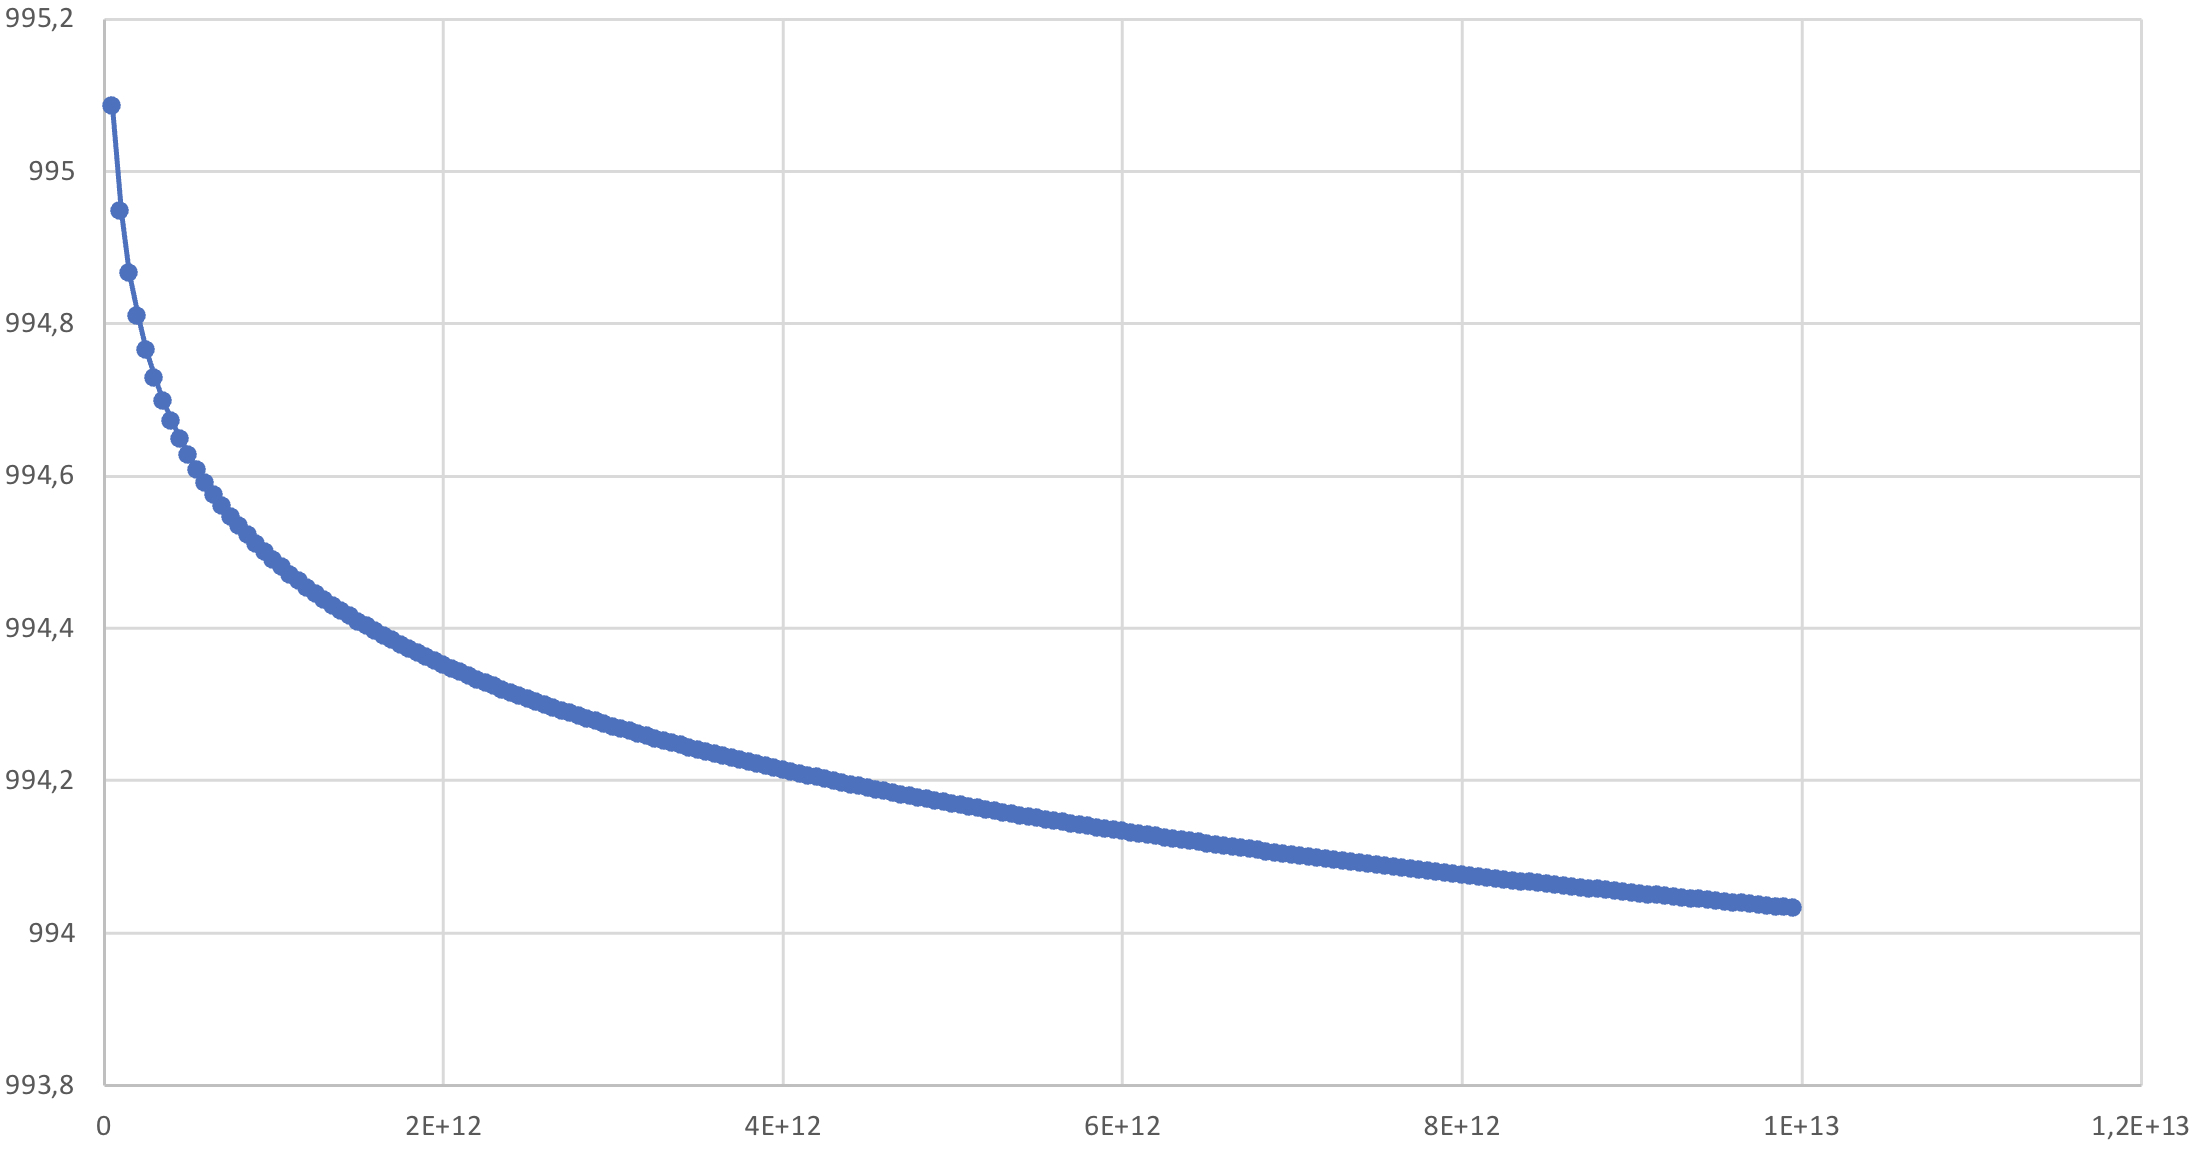
\includegraphics[scale=0.12]{bandwidth_seq.jpeg}
    \centering
\end{figure}

\end{frame}

\begin{frame}
\frametitle{Proof component}
\begin{block} {Theorem A}
\begin{enumerate} [label=(\roman*)]
    \item $m_n$ local averaging estimate with subprobability weights
    \item $m_n$ strongly universal consistent with bounded $Y$
    \item $\exists c < \infty $ : $\forall Y$ with $\ev{Y^2}<\infty : $
\[\limsup_{n \to \infty} \sum_{i=1}^{n}Y_i^2 \int \alpha_{n,i}(x) \mu(\diff{x}) \leq c\ev{Y^2} \ \text{\(\mathbb{P}\)-a.s.}\]
\end{enumerate}
Then $m_n$ is strongly universally consistent.
\end{block}
    
\end{frame}

%-------------------

\section{k-NN Estimates}

\begin{frame}
\frametitle{Strong consistency of the k-NN estimate}
\begin{alertblock}{Theorem 3.1 (strong consistency)}
% Let \(\abs{Y} \leq L\) \(\mathbb{P}\)-a.s. for some \(L < \infty\) and that for each \(x \in \R^d\) the RV \(\norm{X - x}\) is absolutely continuous. If 
% \[k_n \to \infty \quad \text{and} \quad k_n / n \to 0,\]
% then the \(k_n\)-NN regression function estimate is strongly consistent. 
(1) \(\exists L < \infty\) s.t. \(\abs{Y} \leq L\) \(\mathbb{P}\)-a.s. \\
(2) \(\forall x \in \R^d\): \(\norm{X - x}\) absolutely continuous. \\ 
If \[k_n \to \infty \quad \text{and} \quad k_n / n \to 0,\]
\(\implies\) \(k_n\)-NN regression function estimate is strongly consistent. 
\end{alertblock}
\end{frame}

\begin{frame}
\frametitle{Proof components (overview)}
\begin{figure}
    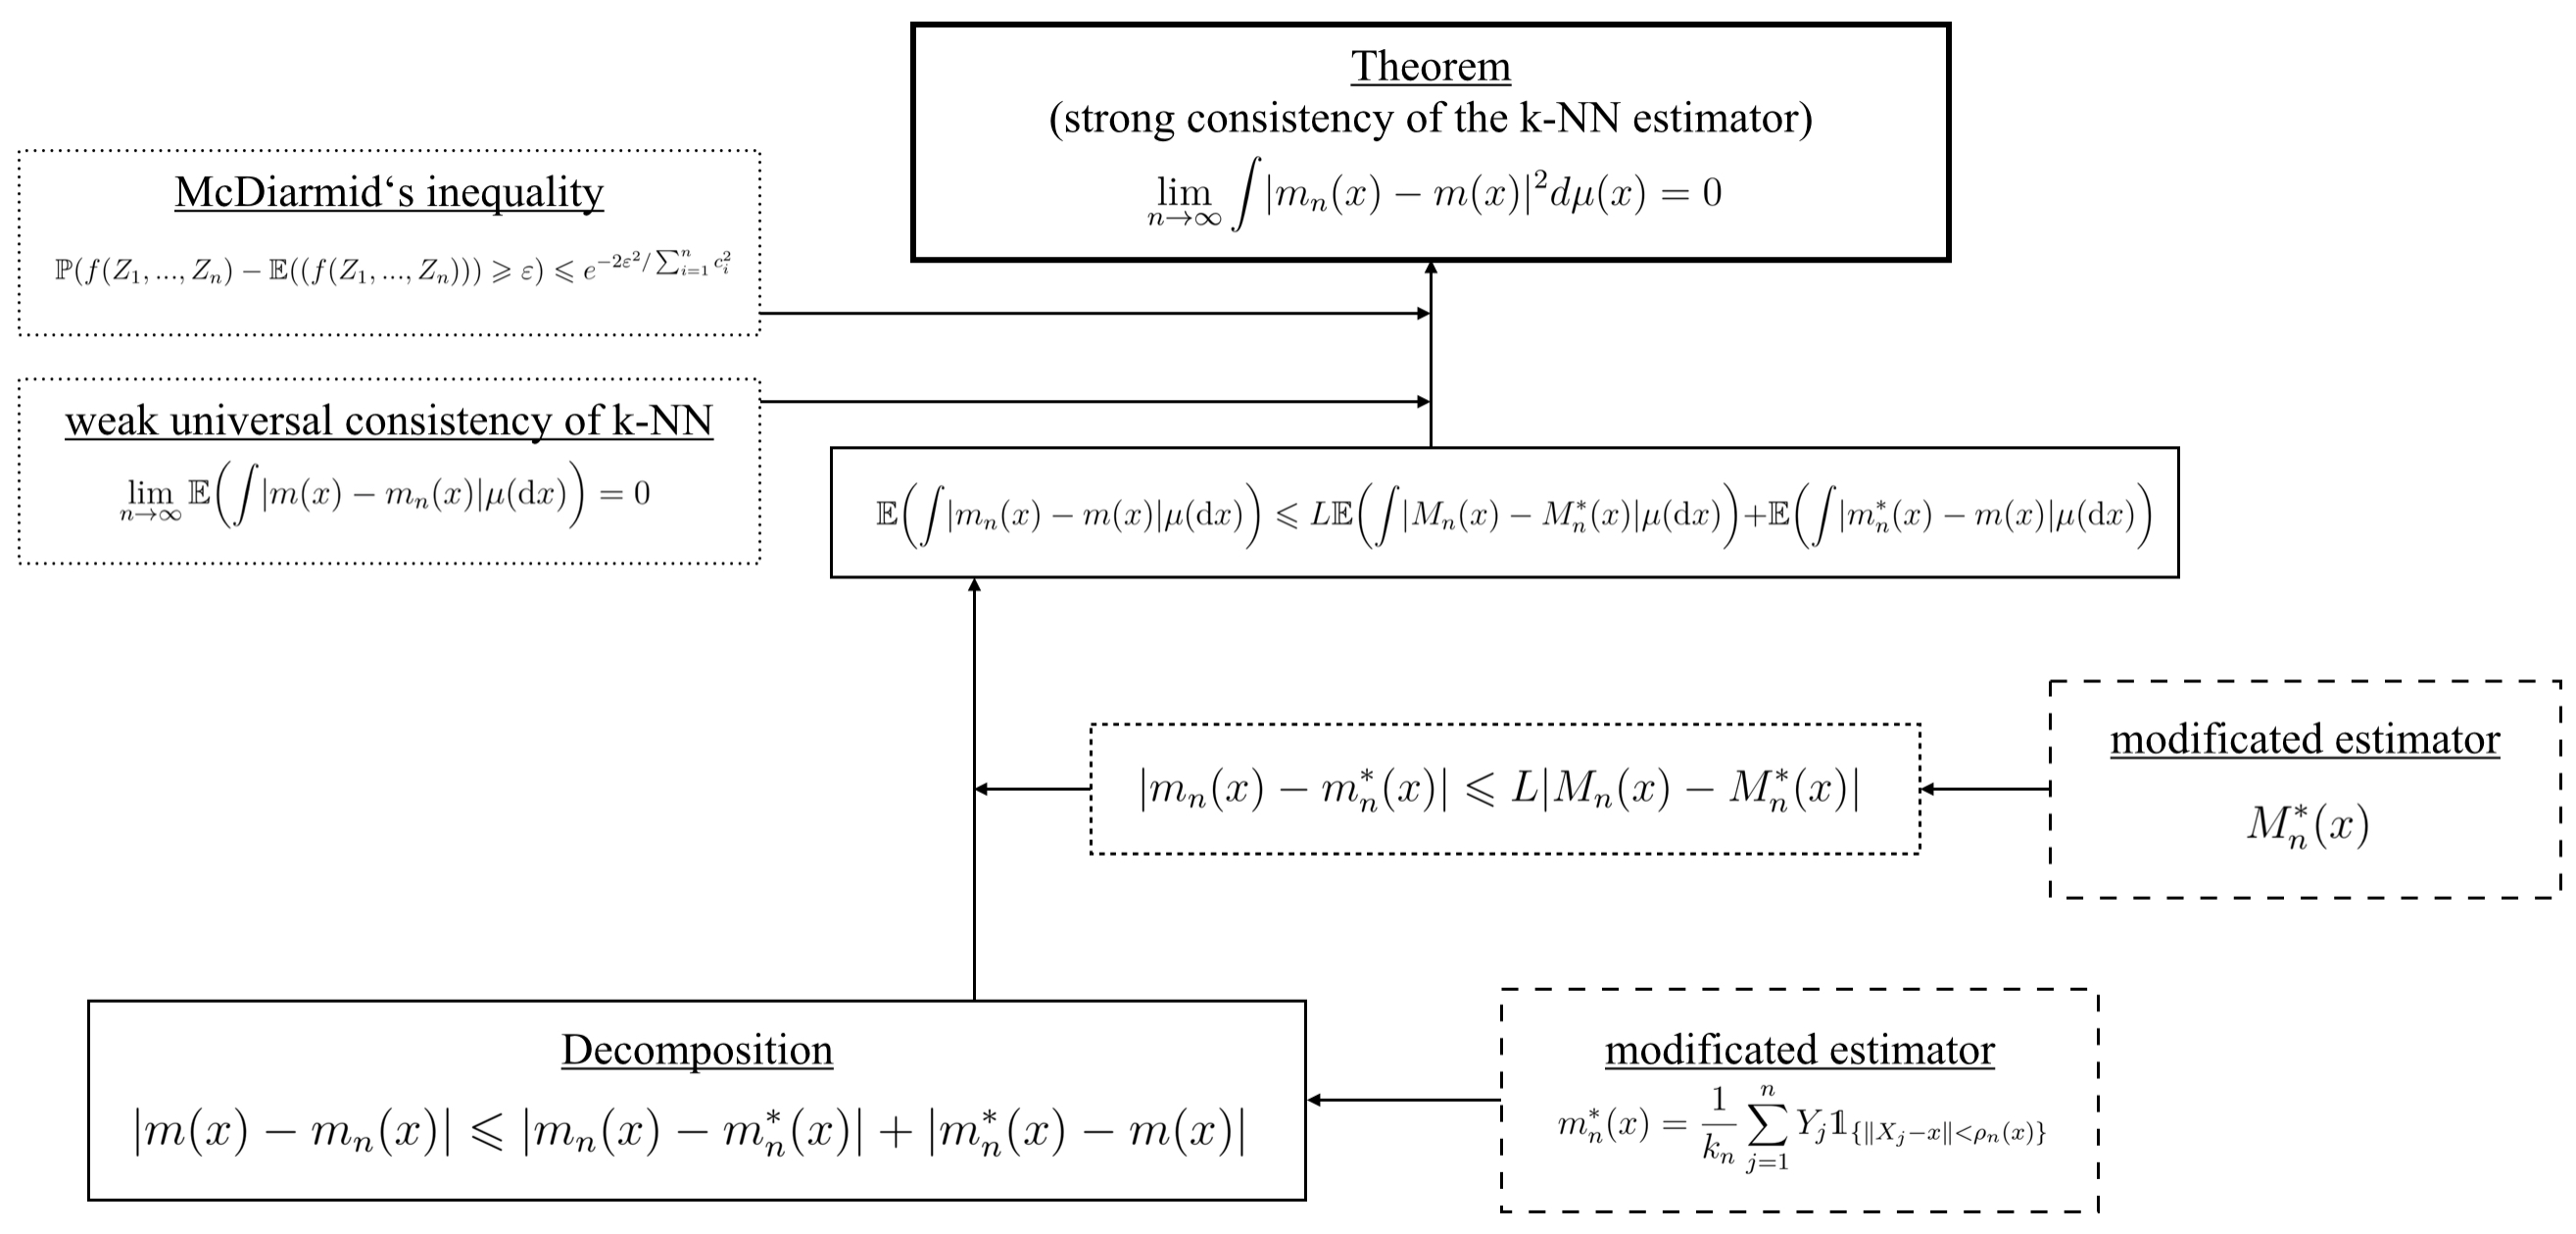
\includegraphics[scale=0.11]{organigramknn.jpeg}
    \centering
\end{figure}
\end{frame}


\begin{frame}
\frametitle{Reminder}
Remembering the cone property
\begin{figure}
    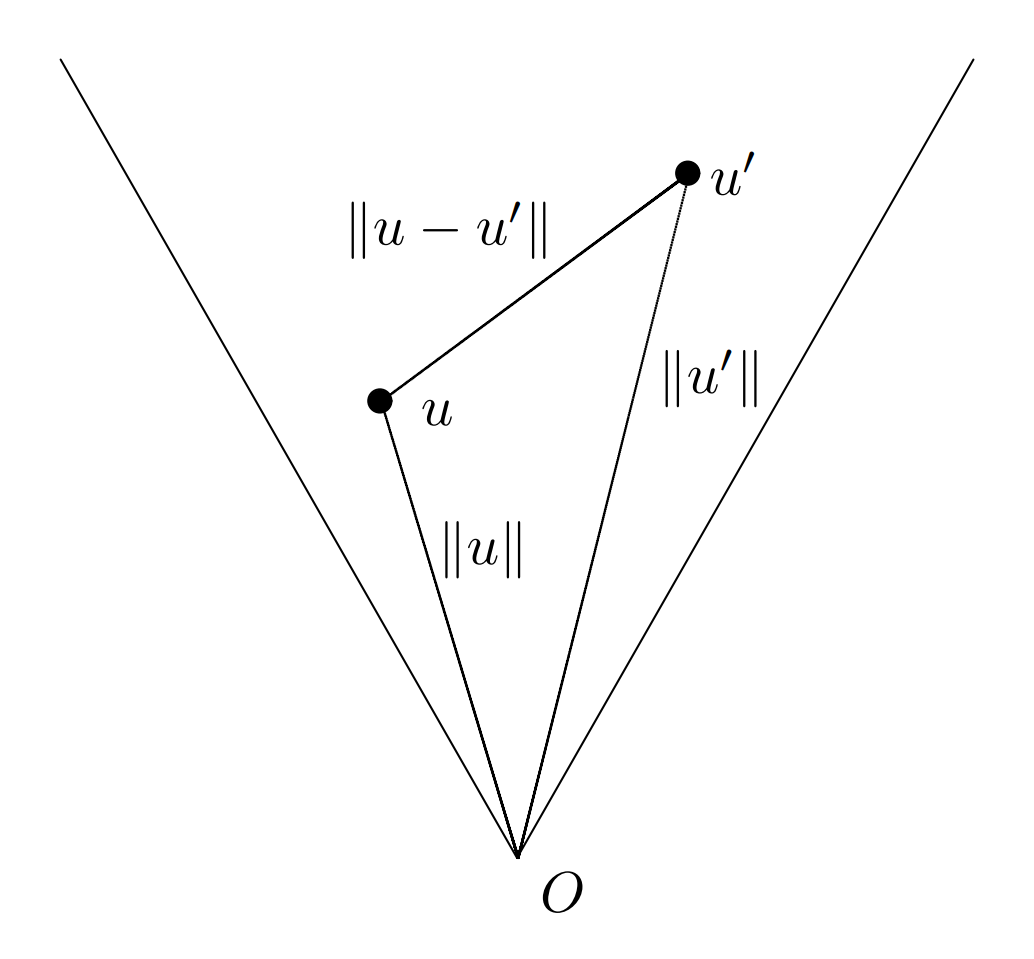
\includegraphics[scale=0.2]{cone_property.png}
    \centering
\end{figure}
\(\norm{u} < \norm{u'} \implies \norm{u - u'} < \norm{u'}\)
\end{frame}

\begin{frame}
\frametitle{Some useful sets}
\begin{block}{Definition ($A_i$)}
Let \(A_i\) be the collection of all \(x \in \R^d\), s.t. \(X_i\) is one of its \(k_n\) nearest neighbors of \(x\) in \(\{X_1, \ldots, X_n\}\).
\end{block}
\end{frame}

\begin{frame}
\frametitle{Some useful sets}
\begin{block}{Definition ($C_{i, j}$)}
Let \(C_j\) be a cone of radius \(\pi/3\), s.t. \(C_1, \ldots, C_{\gamma_d}\) covers \(\R^d\).
We define \(C_{i, j} := X_i + C_j \quad \forall i \in \{1, \ldots, n\} \ \forall j \in \{1, \ldots, \gamma_d\}\).
\end{block}

\begin{block}{Definition ($B_{i, j}$)}
Let \(B_{i, j}\) be the subset of \(C_{i, j}\) consisting of all \(x \in C_{i, j}\) that are among the \(k_n\) nearest neighbors of \(X_i\) in the set
    \[
        \{X_1, \ldots, X_{i-1},X_{i+1}, \ldots, X_n, x\} \cap C_{i, j}. 
    \]
    Equivalently \(B_{i, j}\) is the subset of \(C_{i, j}\) consisting of all \(x\) that are closer to \(X_i\) than the \(k_n\)-th nearest neighbor of \(X_i\) in \(\{X_1, \ldots, X_{i-1}, X_{i+1}, \ldots, X_n\} \cap C_{i, j}\).
\end{block}
\end{frame}

\begin{frame}
\frametitle{Some useful sets}
Example of \(B_{i, j}\) and \(C_{i, j}\) with \(k_n = 2, i = 1\).
\begin{figure}[htbp]
  \centering
  \includesvg[scale=0.43]{bij.svg}
\end{figure}
\end{frame}


\begin{frame}
\frametitle{Strong universal consistency of the k-NN estimate}
\begin{block}{Lemma 3.2 (\(k\)-NN covering)}
If \(x \in A_i\), then \(x \in \bigcup_{j=1}^{\gamma_d} B_{i,j}\), and thus
\[
    \mu(A_i) \leq \sum_{j=1}^{\gamma_d}\mu(B_{i,j}).
\]
\end{block}

\begin{exampleblock}{Proof idea: Cone property!}
Take \(X_l \in C_{i, j}\) that is \(k_n\)-NN of \(X_i\) \\
Then \(\norm{X_l - X_i} < \norm{x - X_i} \implies \norm{X_l - x}< \norm{X_i - x}\) \\
\(x \in A_i \implies X_l \ k_n\)-NN of \(x\)
\(\implies\) there can exist at most \(k_n - 1\) points \(X_l \in C_{i, j}\) closer to \(X_i\) than \(x\).
\(\implies x \in B_{i, j}\)
\end{exampleblock}
\end{frame}

\begin{frame}
\frametitle{Strong universal consistency of the k-NN estimate}
\begin{block}{Lemma 3.3 (\(k\)-NN upper bound for \(B_{i, j}\))}
If \(k_n / \log(n) \to \infty\) and \(k_n / n \to 0\),
\(\forall x \in \R^d\): \(\norm{X - x}\) absolutely continuous
\[
    \implies \limsup_{n \to \infty} \frac{n}{k_n}\max_{1 \leq i \leq n} \mu(B_{i, j}) \leq 2 \quad \text{\(\mathbb{P}\)-a.s.} \quad  \forall j \in \{1, \ldots, \gamma_d\}
\]
\end{block}

\begin{exampleblock}{Proof idea: Borel-Cantelli Lemma}
Show that \(\sum_{n=1}^\infty \pro{\frac{n}{k_n}\max_{1 \leq i \leq n} \mu(B_{i, j}) > 2} < \infty\)
\end{exampleblock}

\end{frame}

\begin{frame}
\frametitle{Strong universal consistency of the k-NN estimate}
\begin{alertblock}{Theorem 3.2 (strong universal consistency)}
%Assume that for each \(x \in \R^d\) the RV \(\norm{X - x}\) is absolutely continuous. If \[k_n / \log n \to \infty \quad \text{and} \quad k_n / n \to 0\] then the \(k_n\)-NN regression function estimate is strongly universal consistent.
\(\forall x \in \R^d\): \(\norm{X - x}\) absolutely continuous. \\
If  \[k_n / \log n \to \infty \quad \text{and} \quad k_n / n \to 0\]
\(\implies\)  \(k_n\)-NN regression function estimate is strongly universally consistent
\end{alertblock}
\end{frame}

\begin{frame}
\frametitle{Proof Sketch SUC}
Only thing to show:
\begin{block} {Theorem A}
\begin{enumerate} [label=(\roman*)]
    \item $m_n$ local averaging estimate with subprobability weights
    \item $m_n$ strongly universal consistent with bounded $Y$
    \item $\exists c < \infty $ : $\forall Y$ with $\ev{Y^2}<\infty : $
\[\limsup_{n \to \infty} \sum_{i=1}^{n}Y_i^2 \int \alpha_{n,i}(x) \mu(\diff{x}) \leq c\ev{Y^2} \ \text{\(\mathbb{P}\)-a.s.}\]
\end{enumerate}
Then $m_n$ is strongly universally consistent.
\end{block}
\end{frame}

\begin{frame}
\frametitle{Proof Sketch SUC}
In our case:
\begin{block} {}
\begin{align*}
    &\quad \sum_{i=1}^{n}Y_i^2 \int \alpha_{n,i}(x) \mu(\diff{x}) \\
    &= \frac{1}{k_n} \sum_{i=1}^{n}Y_i^2 \int \ind{\{\text{\(X_i\) is among the \(k_n\) NNs of \(x\)}\}} \mu(\diff{x}) \\
    &= \frac{1}{k_n} \sum_{i=1}^{n}Y_i^2 \int \ind{\{x \in A_i\}} \mu(\diff{x}) \\
    &= \frac{1}{k_n} \sum_{i=1}^{n}Y_i^2 \mu(A_i) \\
\end{align*}
\end{block}
\end{frame}

\begin{frame}
\frametitle{Proof Sketch SUC}
\begin{block} {}
\begin{align*}
    \frac{1}{k_n} \sum_{i=1}^{n}Y_i^2 \mu(A_i)
    \leq \left(\frac{n}{k_n} \max_{1 \leq i \leq n} \mu(A_i) \right) \frac{1}{n}\sum_{i=1}^{n}Y_i^2
\end{align*}
\end{block}
\end{frame}

\begin{frame}
\frametitle{Proof Sketch SUC}
Utilizing the \(k\)-NN covering Lemma
\begin{block} {}
\begin{align*}
        &\quad \limsup_{n \to \infty} \frac{n}{k_n} \max_{1 \leq i \leq n} \mu(A_i) \\
        &\leq \limsup_{n \to \infty} \frac{n}{k_n} \max_{1 \leq i \leq n} \sum_{j=1}^{\gamma_d} \mu(B_{i, j}) \\
        &\leq \limsup_{n \to \infty} \frac{n}{k_n} \sum_{j=1}^{\gamma_d} \max_{1 \leq i \leq n} \mu(B_{i, j}) \\
        &= \sum_{j=1}^{\gamma_d} \limsup_{n \to \infty} \frac{n}{k_n}  \max_{1 \leq i \leq n} \mu(B_{i, j}) \\
\end{align*}
\end{block}
\end{frame}

\begin{frame}
\frametitle{Proof Sketch SUC}
With our second Lemma:
\begin{block} {}
\begin{align*}
        \sum_{j=1}^{\gamma_d} \limsup_{n \to \infty} \frac{n}{k_n}  \max_{1 \leq i \leq n} \mu(B_{i, j}) 
        \leq \sum_{j=1}^{\gamma_d} 2
        = 2\gamma_d
\end{align*}
\end{block}

\end{frame}

\begin{frame}
\frametitle{Proof Sketch SUC}
And finally by the strong law of large numbers
\begin{block} {}
\begin{align*}
        \limsup_{n \to \infty } \left(\frac{n}{k_n} \max_{1 \leq i \leq n} \mu(A_i) \right) \frac{1}{n}\sum_{i=1}^{n}Y_i^2
        \leq 2\gamma \ev{Y^2} \ \text{\(\mathbb{P}\)-a.s.}
\end{align*}
\end{block}
and we are done.
\end{frame}

\section{Comparison}

\begin{frame}
\frametitle{Where are we?}
\begin{tabularx}{0.98\textwidth} {
  | >{\centering\arraybackslash}X 
  || >{\centering\arraybackslash}X
  | >{\centering\arraybackslash}X 
  | >{\centering\arraybackslash}X | }
 \hline
   & \textbf{Partitioning} & \textbf{Kernel} & \textbf{k-NN} \\ 
 \hline
 \hline
    \textbf{weak} & & & \\
    universal consistency & \checkmark & \checkmark & \checkmark \\
 \hline
    \textbf{strong} & & & \\
    (universal) consistency & \checkmark & \checkmark & \checkmark \\ 
 \hline
\end{tabularx}
\end{frame}

\begin{frame}
\frametitle{Comparison: \\ Strong vs. weak (universal) consistency}

\begin{tabularx}{0.98\textwidth} {
  | >{\centering\arraybackslash}X 
  | >{\centering\arraybackslash}X 
  | >{\centering\arraybackslash}X | }
 \hline
    \multicolumn{3}{|c|}{\textbf{KERNEL ESTIMATE}} \\ 
 \hline
 \hline
    boxed & regular & naive\\
 \hline
    \multicolumn{3}{|c|}{$h_n \to 0$} \\
    \multicolumn{3}{|c|}{$nh_n^d \to \infty$} \\
 \hline
    --&$|Y| \leq L$ in  $\mathbb{P}$ &$h_n \neq h_{n+1}$\\
 \hline
 \multicolumn{1}{c}{$\Downarrow$} & \multicolumn{1}{c}{$\Downarrow$} & \multicolumn{1}{c}{$\Downarrow$}\\ 
 \hline
 \textbf{weak universal} consistency & \textbf{strong} \mbox{consistency} & \textbf{strong universal} consistency\\ \hline
\end{tabularx}



\end{frame}

\begin{frame}
\frametitle{Comparison: \\ Strong vs. weak (universal) consistency}

\begin{tabularx}{0.98\textwidth} {
  | >{\centering\arraybackslash}X 
  | >{\centering\arraybackslash}X 
  | >{\centering\arraybackslash}X | }
 \hline
    \multicolumn{3}{|c|}{\textbf{K-NN ESTIMATE}} \\ 
 \hline
 \hline
    \multicolumn{2}{|c|}{$k_n \to \infty$} & $k_n/log(n) \to \infty$ \\
 \hline
    \multicolumn{3}{|c|}{$k_n/n \to 0$} \\ 
 \hline
    \multicolumn{3}{|c|}{$\pro{ties}=0$} \\ 
 \hline
    -- & $|Y| \leq L$ a.s. & -- \\ 
 \hline
    -- &  \multicolumn{2}{c|}{$\norm{X-x}$ abs. continuous}\\
 \hline
 \multicolumn{1}{c}{$\Downarrow$} & \multicolumn{1}{c}{$\Downarrow$} & \multicolumn{1}{c}{$\Downarrow$}\\ 
 \hline
 \textbf{weak universal} consistency & \textbf{strong} \mbox{consistency} & \textbf{strong universal} consistency\\ \hline
\end{tabularx}

\end{frame}

\section{Programming part}